\section{Redes Bayesianas}

Redes bayesianas sãp uma classe de modelos gráficos que permitem a representação de probabilidades condicionais entre um conjunto dado de variáveis aleatórias $X = {X_1,X_2,...X_p}$ como um grafo acíclico direto (DAG) $G = (V,A)$. Cada nó $v_i \in V$ corresponde a uma variável aleatória $X_i$.

As redes Bayesianas podem ser utilizadas para:
    
    \begin{itemize}
        \item Tomar decisões baseadas em probabilidades.
        \item Decidir quais evidências adicionais devem ser observadas, a fim de obter total conhecimento do domínio.
        \item Realizar uma análise sensitiva para entender quais aspectos do modelo tem maior impacto sobre determinadas variáveis.
        \item Explicar os resultados de uma inferência probabilística.
\end{itemize}
    
\subsection{Propriedades das Redes Bayesianas}

Um exemplo de DAG é mostrado na Figura~\ref{fig:fig75}. Nesse exemplo, a variável $Z$ é condicionada às variáveis $X$ e $Y$.

\begin{figure}[t]
    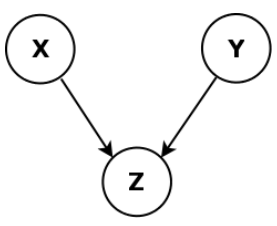
\includegraphics[width=4cm]{fig75.png}
    \centering
    \caption{Representação de probabilidades condicionais um grafo acíclioco direto (DAG).}
    \label{fig:fig75}
\end{figure}

Assim, uma rede Bayesiana consiste:

\begin{itemize}
    \item Um conjunto de variáveis e um conjunto de arcos ligando as variáveis;
    \item Cada variável possui um número limitado de estados mutuamente exclusivos;
    \item As variáveis e arcos formam um grafo dirigido e sem ciclos;
    \item Para cada variável $A$ que possui como pais $B_1, ..., B_n$, existe uma tabela de probabilidade condicional (TPC) $P(A|B_1, ..., B_m)$.
\end{itemize}

Uma rede Bayesiana é a representação de um domínio caso a condição de Markov seja satisfeita. A condição de Markov é definida dessa forma: suponha a distribuição de probabilidade conjunto das variáveis aleatórias em um conjunto de nós $V$ em um DAG $G = (V, E)$. Então, dizemos que $(G, P)$ satisfazem a condição de Markov se cada variável $X \in V, X$ é condicionalmente independente dos nós não descendentes dados os seus pais.

A condição de Markov afirma que as variáveis não-descendentes não fornecem informações adicionais sobre a variável em questão. Considerando $f_X$ e $Pa_X$ o conjunto de filhos e dos pais do nó $X$ respectivamente, e ainda $Pa_{F_{X}}$ como o conjunto dos pais dos descendentes diretos de $X$. O conjunto de nós formados pela união desses três conjuntos é denominado Markov Blanket (ver Figura~\ref{fig:fig76}).

\begin{figure}[t]
    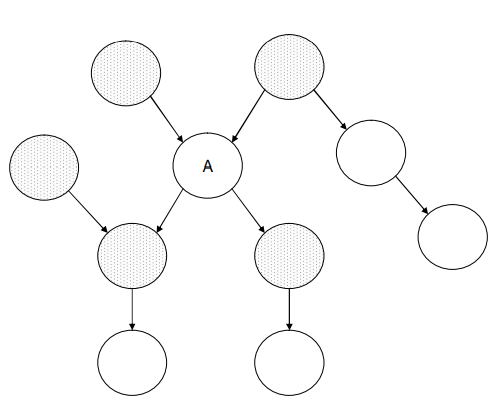
\includegraphics[width=8cm]{fig76.png}
    \centering
    \caption{Os nós preenchidos com cinza representam o conjunto de nós conforme critério Markov Blanket.}
    \label{fig:fig76}
\end{figure}

Se uma rede Bayesiana satisfaz a condição de Markov, então a sua distribuição de probabilidade conjunto é igual ao produto das probabilidades condicionais de todos os nós dado os valores de seus pais.

\begin{equation}
    Pr(X_1, ..., X_n) = \prod_{i=1}^{n}{Pr(X_i | pa(X_i))}
\end{equation}

Através das propriedades markovianas, podemos considerar que a variável aleatória é independente de outra se não existe entre as variáveis analisadas um grupo específico de variáveis, podendo ser um grupo de evidências. Nesse caso, surge o conceito de d-separação. Para defini-la, consideremos alguns tipos de conexões. Seja $X$, $Z$, e $Y$ variáveis de uma rede Bayesiana $(\xi, V)$, definimos alguns tipos de conexão:

\begin{enumerate}
    \item Se $X \rightarrow Z \rightarrow Y$. temos um relacionamento head-to-tail;
    \item Se $X \leftarrow Z \rightarrow Y$, temos um relacionamento tail-to-tail;
    \item Se $X \rightarrow Z \leftarrow Y$, temos um relacionamento head-to-head.
\end{enumerate}

\begin{figure}[t]
    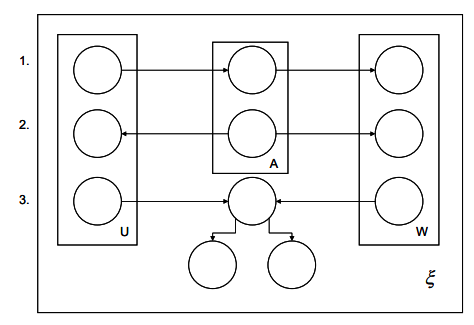
\includegraphics[width=8cm]{fig77.png}
    \centering
    \caption{A independência entre as variáveis aleatórias analisadas em relação ao tipo de conexão.}
    \label{fig:fig77}
\end{figure}

Dada a rede Bayesiana $(\xi, V)$, representada na Figura~\ref{fig:fig77}. Podemos definir $A \subset V$, sendo $X$ e $Y \in V - A$. Desta forma, para os casos 1 e 2, se consideramos que $Z \in A$, a variável $Z$ bloqueará o caminho entre $X$ e $Y$. Para o caso 3, se consideramos que $Z$ e seus descendentes $\notin A$, a variável $Z$ bloqueará o caminho entre $X$ e $Y$. Se o caminho entre duas variáveis, ou conjunto de variáveis, é bloqueado, dizemos que essas variáveis, ou conjuntos, são d-separados.

\subsection{Inferência em Redes Bayesianas}

Pode-se extrair conhecimento da rede Bayesiana através de um processo de inferência. Existem vários métodos para realização de inferência. Inferências podem ser realizadas sobre redes Bayesianas em 04 maneiras distintas:

\begin{itemize}
    \item Diagnósticos: partindo dos efeitos para as causas.
    \item Causa: partindo das causas para os efeitos.
    \item Intercausal: entre causas de um efeito comum.
    \item Mistas: combinação de dois ou mais tipos descritos acima.
\end{itemize}

A figura~\ref{fig:fig72} ilustra essas 04 formas de raciocínio.

\begin{figure}[t]
    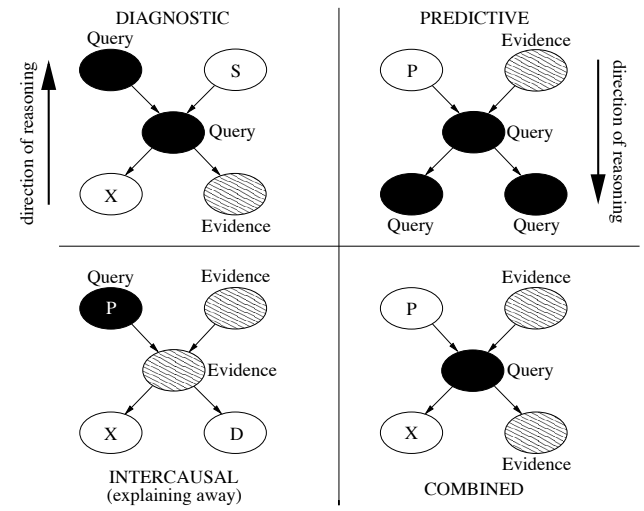
\includegraphics[width=11cm]{fig72.png}
    \centering
    \caption{Tipos de raciocínio presentes em uma rede Bayesiana.}
    \label{fig:fig72}
\end{figure}

\subsection{Estimação de Parâmetros das Redes Bayesianas}

A estimação de parâmetros é a parte final da modelagem por redes bayesianas. Após a seleção das variáveis ter sido feita e a estrutura da rede ter sido fixada, precisamos agora conhecer as probabilidades condicionais de cada variável aleatória, dado os valores de seus antecessores. Para essa tarefa existem várias abordagens. Vamos descrever duas: estimação por máxima verossimilhança (MAP), e estimação por aprendizado sequencial, também conhecida como método bayesiano.

Considerando uma base de dados $D$ completa, e considerando meta-independência global e meta-independência local.

blábláblá...

\subsection{Decisão com Redes Bayesianas}

blábláblá...
